\section{Case Study}
\label{sec:caseStudy}
%\vspace{-4mm}
\begin{figure}[th]
\centering
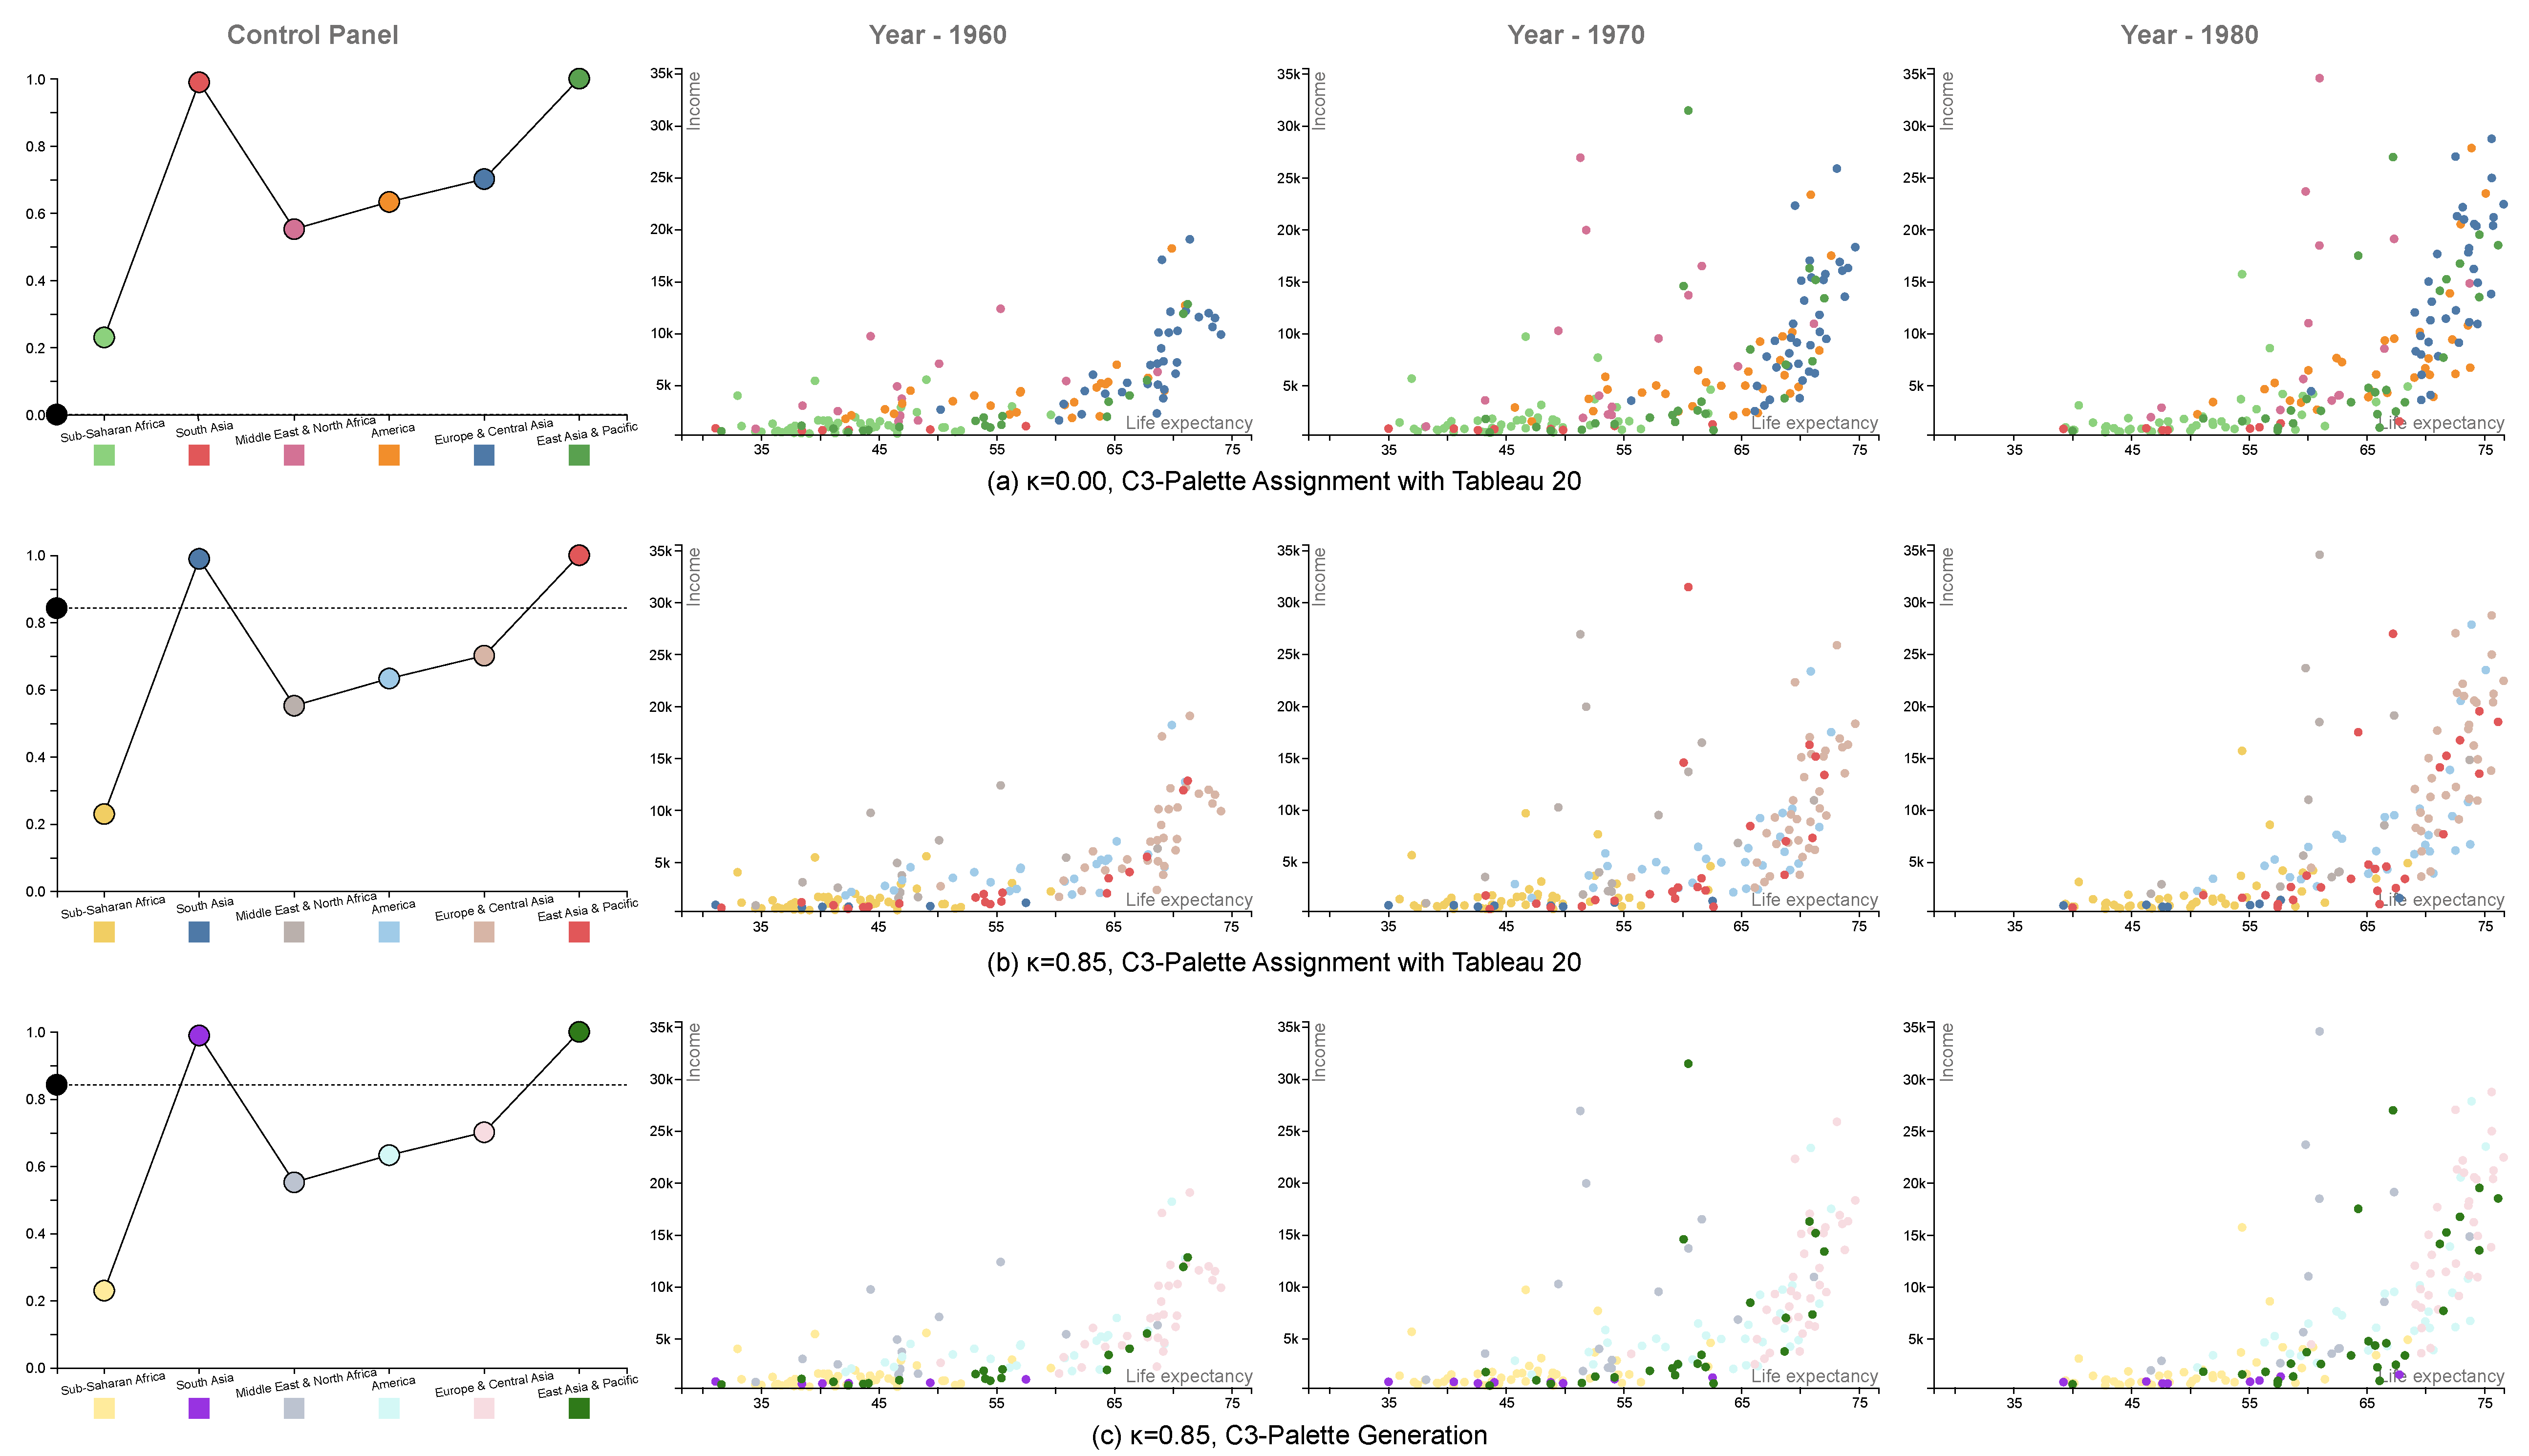
\includegraphics[width=\linewidth]{case-study.pdf}
\caption{Gapminder dataset: (a) Result generated by default setting for given palette; (b) User-specified $\kappa$ value for popping out classes; (c) Automatic palette generation for achieving a better discriminablity.}
\label{fig:casestudy}
\vspace{-4mm}
\end{figure}
We conducted a case study with a real world data, which is well-known for the use in Gapminder~\cite{gapminder}, to evaluate the usability of our system.
We choose life expectancy and income as the x axis and y axis, respectively. And we use world regions as the class label. As shown in Fig.~\ref{fig:casestudy}, due to the limit space, we only show three years. And to make it easy to read, we removed the points with a much larger x value or y value.

We first used the default settings of our system to automatically produce a color assignment result based on Tableau 20 palette for assigning colors to different objects in the dataset, see Fig.~\ref{fig:casestudy}(a). Since $\kappa$ is $0$ and all the classes are changed, each class is assigned with a salient color to make it more distinguishable. This result is similar to \emph{Optimized Assignment}~\cite{Wang2018} while our result considers the different importance of classes, i.e., larger importance value has a more salient color.
Then we want to explore the two classes with the largest change degree, thus we move the $\kappa$ control point(the black circle in control panel) to a larger value, as shown in Fig.~\ref{fig:casestudy}(b). Now we can see the largest changed classes more clearly. But the visual separability between the classes with lower $\kappa$ value is small, such as the color of \emph{Middle East \& North Africa} and \emph{Europe \& Central Asia}. We further generate the result by our palette generation method which has a better performance on discriminability, see Fig.~\ref{fig:casestudy}(c).
Through our exploration, we found that \emph{South Asia} should not have a large change degree. This result is caused by our default class importance measure which sets point number change a larger weight in Eq.~\ref{eq:cm}, this is done due to the previous evaluation result that point number change is harder to distinguish than point position change.

\begin{figure}[h]
\centering
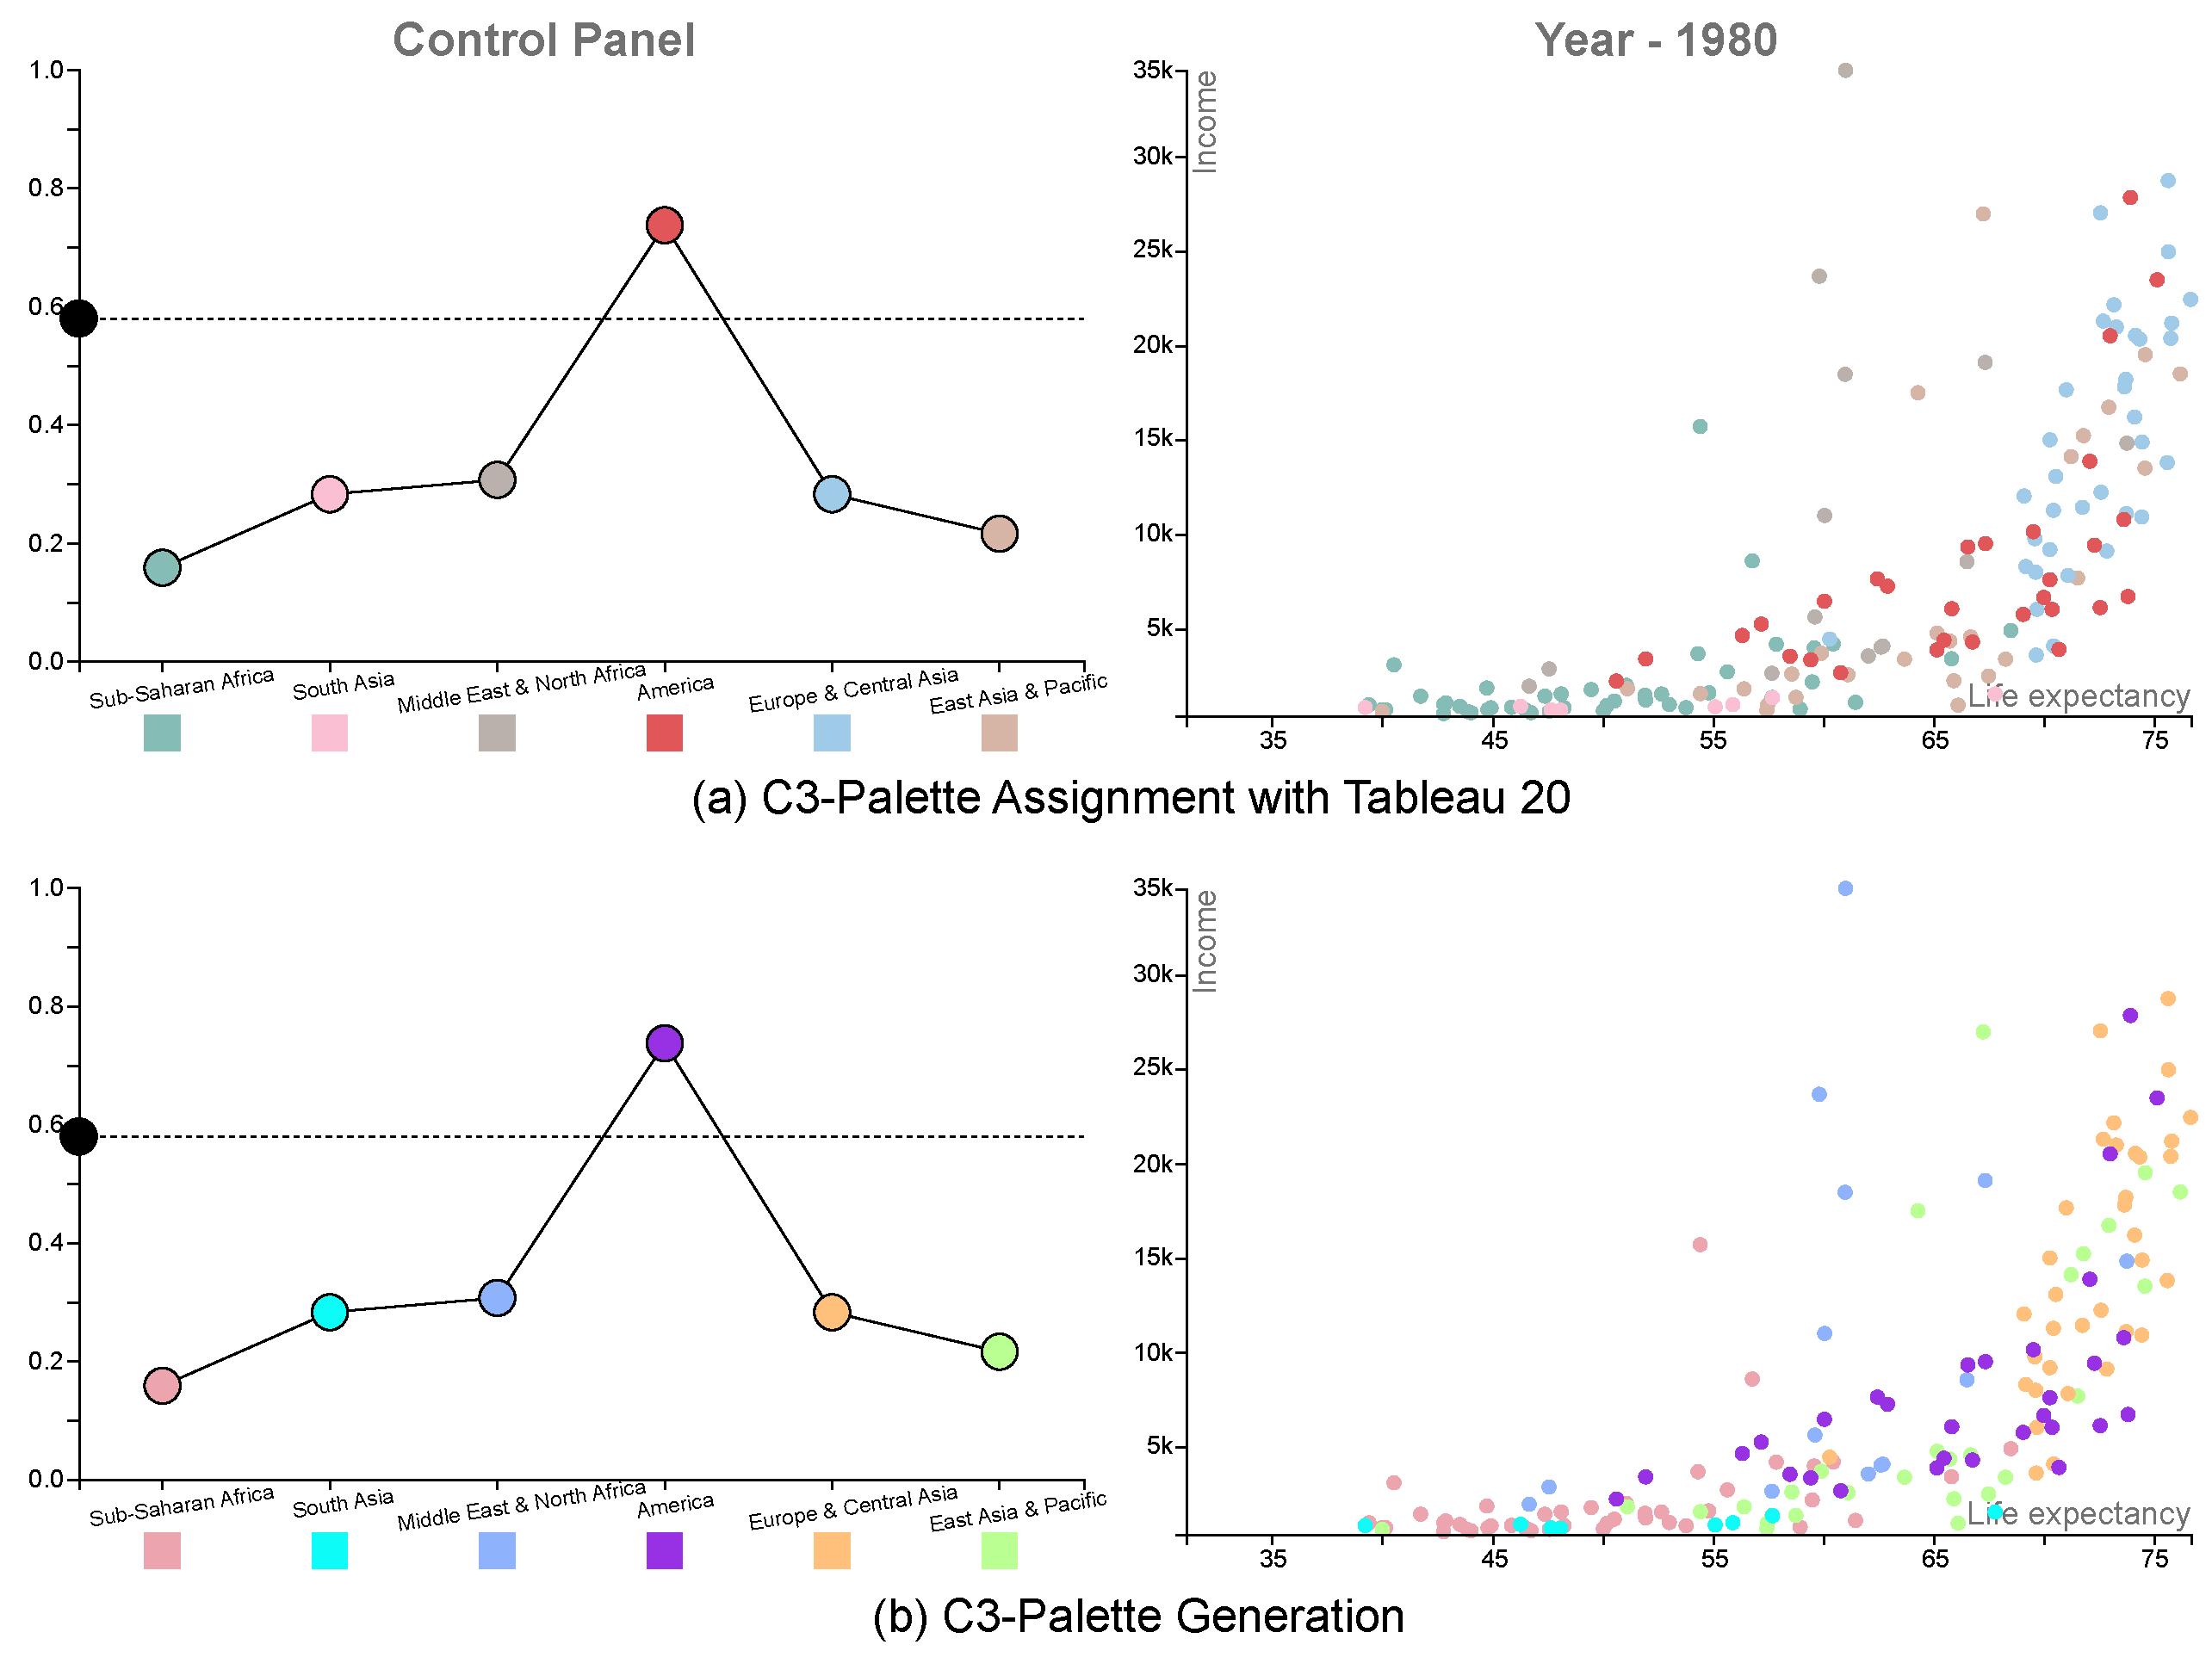
\includegraphics[width=0.8\linewidth]{interaction.pdf}
\caption{Manually define the class importance in the control panel: (a) Result generated based on given palette; (b) Automatic palette generation.}
\label{fig:casestudyinteraction}
\vspace{-4mm}
\end{figure}

Our system also supports manually class importance adjustment, we illustrate this in Fig.~\ref{fig:casestudyinteraction}. For example, we are interested in \emph{America}, thus we can increase the importance value of the corresponding circle and meanwhile, decrease other classes' importance value until lower than $\kappa$. We show both assignment result for user provided palette and automatic palette generation result. It's obvious that both results highlight the interested class while palette generation method leads to a much better visual separability between different classes.

